\section{Durchführung}
\label{sec:Durchführung}

Die Dampfdruckkurve wird bestimmt in zwei Bereichen.
Einmal wird in einem Bereich zwischen ca. \qty{30}{\milli\bar} und \qty{1000}{\milli\bar} gemessen.
Danach in einem Hochdruckbereich von \qty{1}{\bar} bis \qty{15}{\bar}.
Im folgenden werden die einzelnen Methoden erläutert.

\subsection{Messungen im Niedrigdruckbereich unter \qty{1}{\bar}} % (fold)
\label{sub:M_Niedrigdruckbereich}
In einem Druckbereich bis $\qty{1}{\bar}$ kann der Aufbau in \autoref{fig:Abb_3} benutzt werden.
\begin{figure}[H]
    \centering
    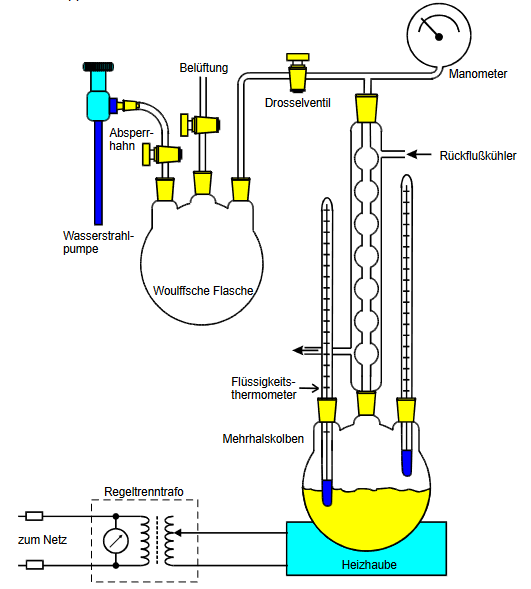
\includegraphics[width=0.7\textwidth]{build/Abb_3.PNG}
    \caption {Aufbau zur Messung unter $\qty{1}{\bar}$.\cite{v203}}
    \label{fig:Abb_3}
\end{figure}
Vor der Messung muss der Aufbau evakuiert werden.
Zum Beispiel mit einer Wasserstrahlpumpe, dafür muss das Belüftungsventil geschlossen sein und der Absperrhahn und das Drosselventil muss geöffnet sein.
Die richtige Messung beginnt, wenn der Enddruck der Evakuierung erreicht wird.
Dieser ist abhängig von der Leitungswassertemperatur.
Die Woulffsche Flasche verhindert, dass kaltes Wasser kaltes Wasser in die erhitzte und evakuiert Flasche eindringt, nach dem Abdrehen der Leitungswasserzufuhr.
Bevor die Wasserstrahlpumpe muss der Absperrhahn geschlossen werden.
Nun beginnt die Messung.
Der Mehrhalskolben mit der Flüssigkeit wird erhitzt und der Rückflusskühler muss während der ganzen Messung mit Leitungswasser durchflossen werden.
Dies dient dazu dass die aufsteigenden Dämpfe kondensieren und nicht ins Mannometer gelangen, was den Druck misst.
Während der Messung wird die Temperatur am Thermometer abgelesen und zu den Drücken in eine Tabelle geschrieben.
Die Menge des Kühlwassers muss bei steigender Temperatur verringert werden.
% subsection M_Niedrigdruckbereich (end)

\subsection{Messungen im Hochdruckbereich über \qty{1}{\bar}} % (fold)
\label{sub:M_Hochdruckbereich}
In einem Druckbereich ab \qty{1}{\bar} muss eine anderer Aufbau benutzt werden, wie zum Beispiel \autoref{fig:Abb_4}.
\begin{figure}[H]
    \centering
    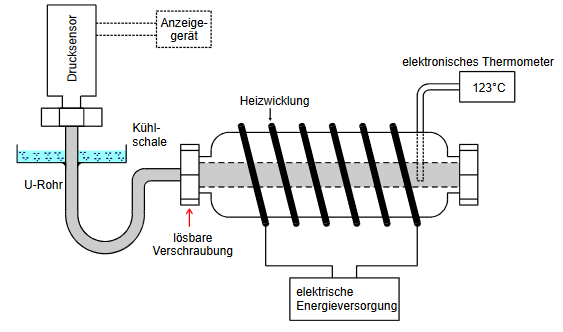
\includegraphics[width=0.7\textwidth]{build/Abb_4.PNG}
    \caption {Aufbau zur Messung über $\qty{1}{\bar}$.\cite{v203}}
    \label{fig:Abb_4}
\end{figure}
Die Apparatur besteht aus einem durchnbohrten Stahlbolzen, wobei in dem Hohlraum destilliertes und entgastes Wasser gefüllt ist.
Einem U-Rohr, einem Drucksensor und einem Thermometer.
Außerdem ist der Stahlzylinder umgeben von einer Heizwicklung, der den Stahlbolzen langsam aufheizt.
Wärhend der Messung werden die Temperatur und der Druck immer wieder abgelesen und in eine Tabelle geschrieben.
% subsection Messungen im Hochdruckbereich über \ (end)